\section{Strategie-Einheit}

\begin{frame}
	\frametitle{Übersicht}
	
\end{frame}

\begin{frame}
	\frametitle{Aufgaben (\textit{Jobs})}
	
	\centering
	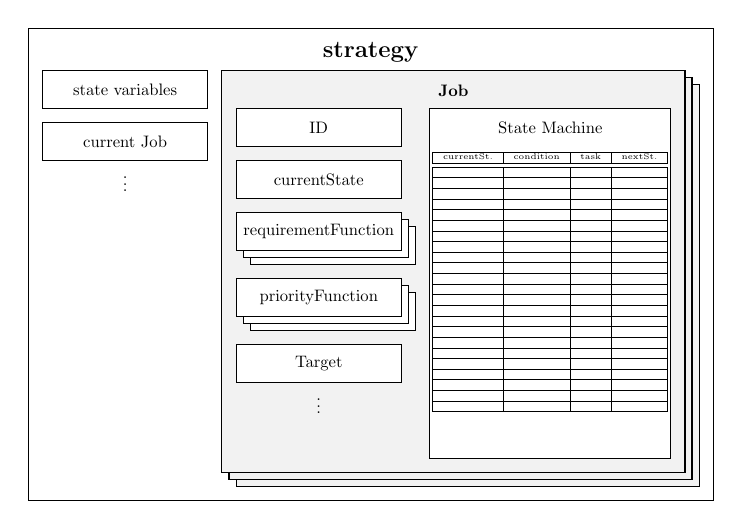
\begin{tikzpicture} [scale=0.6, transform shape]
		\coordinate (strategySize) at (14.5,10);
		\def\top{9.4};
		\def\sep{0.3};
		\def\varHeight{0.8};
		\def\varWidth{3.5};
		\def\jobHeight{8.5};
		\def\jobWidth{9.8};
		\def\jobTop{8.3};
		\def\fsmHeight{\jobTop+3*\sep};
		\def\fsmWidth{\jobWidth-4*\sep-\varWidth};
		\def\fsmText{2.55};
		
		\coordinate (jobStart) at (\sep+\varWidth+\sep, \top-\sep);
		\draw (0,0) rectangle (strategySize) node[pos=0.5, shift={(0, 4.5)}]{\Large \textbf{strategy}}; %strategy box
		
		%strategy components
		\draw (\sep, \top-\sep-0*\sep-0*\varHeight) rectangle ++(\varWidth, -\varHeight) node[pos=0.5]{state variables};
		\draw (\sep, \top-\sep-1*\sep-1*\varHeight) rectangle ++(\varWidth, -\varHeight) node[pos=0.5]{current Job};
		\draw (\sep, \top-\sep-1*\sep-2*\varHeight) [draw=none] rectangle ++(\varWidth, -\varHeight) node[pos=0.5]{$\vdots$};
		
		%jobs
		\draw (jobStart) [shift={(1*\sep, -1*\sep)}, fill=gray!10] rectangle ++(\jobWidth, -\jobHeight);
		\draw (jobStart) [shift={(0.5*\sep, -0.5*\sep)}, fill=gray!10] rectangle ++(\jobWidth, -\jobHeight);
		\draw (jobStart) [shift={(0*\sep, -0*\sep)}, fill=gray!10] rectangle ++(\jobWidth, -\jobHeight) node[pos=0.5, shift={(0, 0.45*\jobHeight)}] {\textbf{Job}};
		
		%job content
		\begin{scope} [shift={(\sep+\varWidth+\sep+\sep, \jobTop)}]
		\draw (0,-0*\varHeight-0*\sep) [fill=white] rectangle ++(\varWidth, -\varHeight) node[pos=0.5] {ID};
		
		\draw (0,-1*\varHeight-1*\sep) [fill=white] rectangle ++(\varWidth, -\varHeight) node[pos=0.5] {currentState};
		
		\draw (1*\sep,-2*\varHeight-3*\sep) [fill=white] rectangle ++(\varWidth, -\varHeight);
		\draw (0.5*\sep,-2*\varHeight-2.5*\sep) [fill=white] rectangle ++(\varWidth, -\varHeight);
		\draw (0,-2*\varHeight-2*\sep) [fill=white] rectangle ++(\varWidth, -\varHeight) node[pos=0.5] {requirementFunction};
		
		\draw (1*\sep,-3*\varHeight-5*\sep) [fill=white] rectangle ++(\varWidth, -\varHeight);
		\draw (0.5*\sep,-3*\varHeight-4.5*\sep) [fill=white] rectangle ++(\varWidth, -\varHeight);
		\draw (0,-3*\varHeight-4*\sep) [fill=white] rectangle ++(\varWidth, -\varHeight) node[pos=0.5] {priorityFunction};
		
		\draw (0,-4*\varHeight-6*\sep) [fill=white] rectangle ++(\varWidth, -\varHeight) node[pos=0.5] {Target};
		
		\draw (0,-5*\varHeight-6*\sep) [draw=none] rectangle ++(\varWidth, -\varHeight) node[pos=0.5]{$\vdots$};
		
		\begin{scope} [shift={(\varWidth+2*\sep, 0)}]
		
		\draw (0,0) [fill=white] rectangle ++(\fsmWidth, -\fsmHeight);
		\node [shift={(\fsmText, -0.4)}] {State Machine};
		\node [shift={(\fsmText, -0.8)}, anchor=north] {
			\tiny
			\begin{tabular}{|c|c|c|c|}
			\hline
			currentSt. & condition & task & nextSt. \\ \hline \hline
			& & & \\ \hline
			& & & \\ \hline
			& & & \\ \hline
			& & & \\ \hline
			& & & \\ \hline
			& & & \\ \hline
			& & & \\ \hline
			& & & \\ \hline
			& & & \\ \hline
			& & & \\ \hline
			& & & \\ \hline
			& & & \\ \hline
			& & & \\ \hline
			& & & \\ \hline
			& & & \\ \hline
			& & & \\ \hline
			& & & \\ \hline
			& & & \\ \hline
			& & & \\ \hline
			& & & \\ \hline
			& & & \\ \hline
			& & & \\ \hline
			& & & \\ \hline
			\end{tabular}
		};
		
		\end{scope}
		
		\end{scope}
	
	\end{tikzpicture}
\end{frame}

\begin{frame}
	\frametitle{Pfadsuche und Spielfeld}
	\vspace{-1.5em}
	\only<1>{\begin{figure}\includegraphics[scale=0.035]{../images/spielfeld/playingAreaPlain.pdf}\end{figure}}	\only<2>{\begin{figure}\includegraphics[scale=0.035]{../images/spielfeld/playingAreaAreas.pdf}\end{figure}}	\only<3>{\begin{figure}\includegraphics[scale=0.035]{../images/spielfeld/playingAreaGraph.pdf}\end{figure}}
	\only<4>{\begin{figure}\includegraphics[scale=0.035]{../images/spielfeld/playingAreaPath1.pdf}\end{figure}}
	\only<5>{\begin{figure}\includegraphics[scale=0.035]{../images/spielfeld/playingAreaPath2.pdf}\end{figure}}
	\only<6>{\begin{figure}\includegraphics[scale=0.035]{../images/spielfeld/playingAreaPath3.pdf}\end{figure}}
	
\end{frame}

\begin{frame}
	\frametitle{\textit{collision handling}}
	\vspace{-1.5em}
	\only<1>{\begin{figure}\includegraphics[scale=0.035]{../images/spielfeld/playingAreaPath4.pdf}\end{figure}}
	\only<2>{\begin{figure}\includegraphics[scale=0.035]{../images/spielfeld/playingAreaPath5.pdf}\end{figure}}
	\only<3>{\begin{figure}\includegraphics[scale=0.035]{../images/spielfeld/playingAreaPath6.pdf}\end{figure}}
\end{frame}

\begin{frame}
	\frametitle{Erkentnisse und Ergebnis}
	
\end{frame}